\documentclass{article}
\usepackage{tikz}
\usetikzlibrary{shapes.geometric, arrows.meta}

% Define styles for nodes and arrows
\tikzset{
    node style/.style={draw, rectangle, rounded corners, minimum width=2cm, minimum height=1cm},
    arrow style/.style={->, thick, >=Stealth[black]}
}

\begin{document}

\begin{figure}[h]
    \centering
    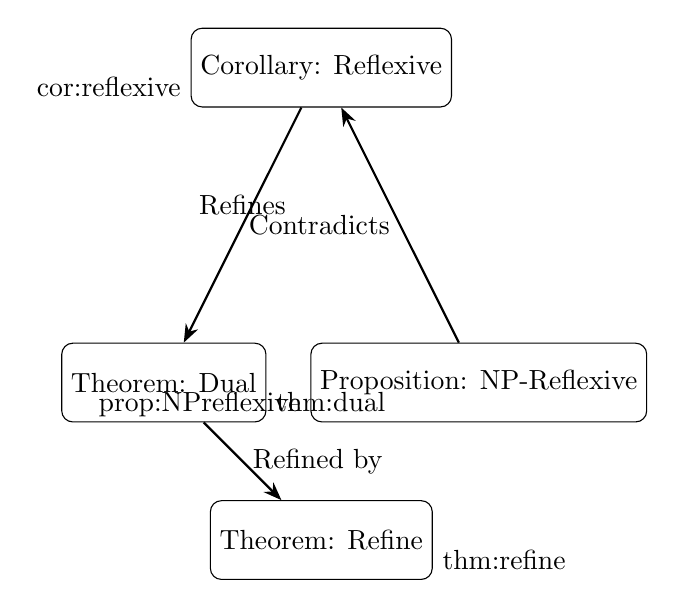
\begin{tikzpicture}
        % Nodes representing theorems and propositions
        \node[node style] (reflexive) at (0,3) {Corollary: Reflexive};
        \node[node style] (dual) at (-2,-1) {Theorem: Dual};
        \node[node style] (NPreflexive) at (2,-1) {Proposition: NP-Reflexive};
        \node[node style] (refine) at (0,-3) {Theorem: Refine};

        % Arrows indicating relationships between nodes
        \draw[arrow style] (reflexive) -- node[above] {Refines} (dual);
        \draw[arrow style] (dual) -- node[right] {Refined by} (refine);
        \draw[arrow style] (NPreflexive) -- node[left] {Contradicts} (reflexive);

        % Adding labels for references
        \node[below left] at (reflexive.west) {\cref{cor:reflexive}};
        \node[below right] at (dual.east) {\cref{thm:dual}};
        \node[below left] at (NPreflexive.west) {\cref{prop:NPreflexive}};
        \node[below right] at (refine.east) {\cref{thm:refine}};
    \end{tikzpicture}
    \caption{Relationships among main results}
    \label{fig:main_results}
\end{figure}

\end{document}